%
% wft.tex -- rectangles for windowed fourier coefficients
%
% (c) 2019 Prof Dr Andreas Müller, Hochschule Rapperswil
%
\documentclass[tikz]{standalone}
\usepackage{amsmath}
\usepackage{times}
\usepackage{txfonts}
\usepackage{pgfplots}
\usepackage{csvsimple}
\usetikzlibrary{arrows,intersections,math}
\begin{document}
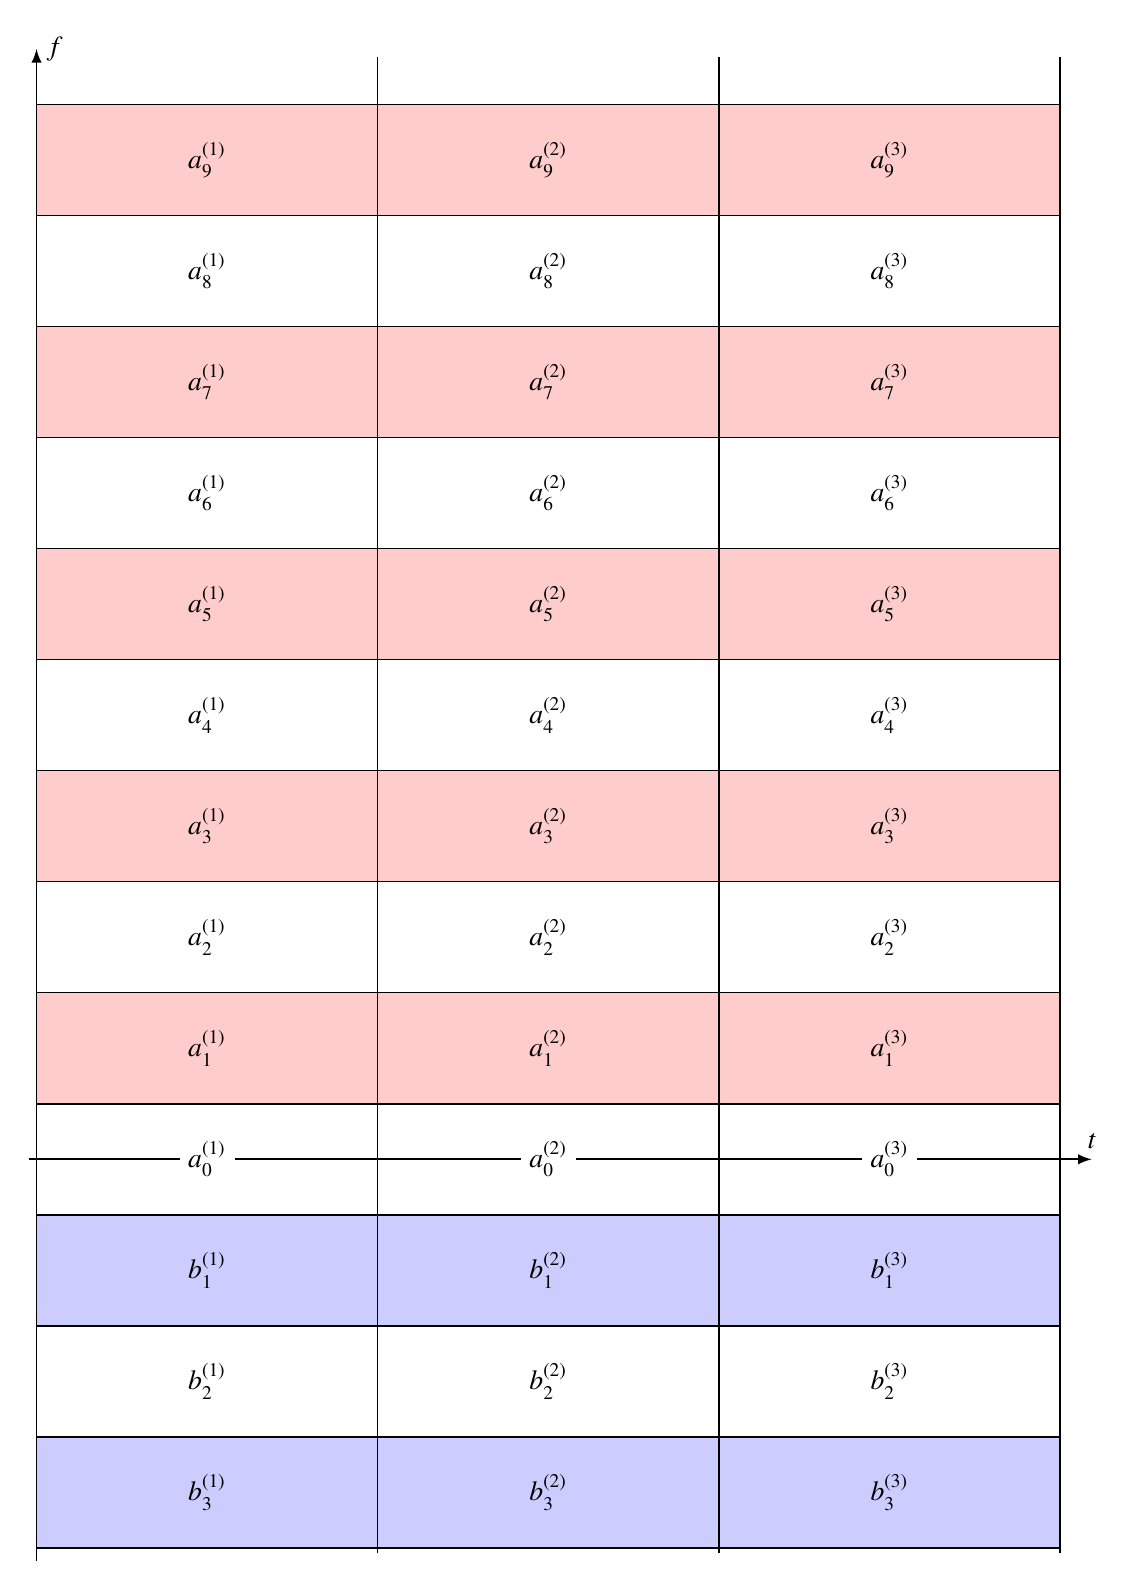
\begin{tikzpicture}[>=latex]

\pgfmathparse{3*0.47}
\xdef\h{\pgfmathresult}
\def\w{13}

\pgfmathparse{14/\h}
\xdef\maxy{\pgfmathresult}
\pgfmathparse{-5/\h}
\xdef\miny{\pgfmathresult}

\foreach \y in {1,3,...,{\maxy}}{
	\fill[color=red!20] (0,{(\y-0.5)*\h})--({\w},{(\y-0.5)*\h})
		--({\w},{(\y+0.5)*\h})--(0,{(\y+0.5)*\h})--cycle;
}

\foreach \y in {1,...,{\maxy}}{
	\draw[line width=0.5pt] (0,{(\y+0.5)*\h})--({\w},{(\y+0.5)*\h});
	\node at ({1*\w/6},{\y*\h}) {$\mathstrut a_{\y}^{(1)}$};
	\node at ({3*\w/6},{\y*\h}) {$\mathstrut a_{\y}^{(2)}$};
	\node at ({5*\w/6},{\y*\h}) {$\mathstrut a_{\y}^{(3)}$};
}

\foreach \y in {1,3,...,{-\miny}}{
	\fill[color=blue!20] (0,{(-\y-0.5)*\h})--({\w},{(-\y-0.5)*\h})
		--({\w},{(-\y+0.5)*\h})--(0,{(-\y+0.5)*\h})--cycle;
}

\foreach \y in {1,2,...,{-\miny}}{
	\draw[line width=0.5pt] (0,{(-\y-0.5)*\h})--(\w,{(-\y-0.5)*\h});
	\node at ({1*\w/6},{-\y*\h}) {$\mathstrut b_{\y}^{(1)}$};
	\node at ({3*\w/6},{-\y*\h}) {$\mathstrut b_{\y}^{(2)}$};
	\node at ({5*\w/6},{-\y*\h}) {$\mathstrut b_{\y}^{(3)}$};
}

\draw[->,line width=0.7pt] (-0.1,0)--(13.4,0) coordinate[label={$t$}];
\draw[->,line width=0.7pt] (0,-5.1)--(0,14.1) coordinate[label={right:$f$}];

\fill[color=white] ({1*\w/6-0.35},{-\h/2})--({1*\w/6+0.35},{-\h/2})
	--({1*\w/6+0.35},{\h/2})--({1*\w/6-0.35},{\h/2})--cycle;
\fill[color=white] ({3*\w/6-0.35},{-\h/2})--({3*\w/6+0.35},{-\h/2})
	--({3*\w/6+0.35},{\h/2})--({3*\w/6-0.35},{\h/2})--cycle;
\fill[color=white] ({5*\w/6-0.35},{-\h/2})--({5*\w/6+0.35},{-\h/2})
	--({5*\w/6+0.35},{\h/2})--({5*\w/6-0.35},{\h/2})--cycle;

\draw[line width=0.7pt] (0,{\h/2})--({\w},{\h/2});
\draw[line width=0.7pt] (0,{-\h/2})--({\w},{-\h/2});

\draw[line width=0.5pt] ({\w},-5)--({\w},14);
\draw[line width=0.5pt] ({\w/3},-5)--({\w/3},14);
\draw[line width=0.5pt] ({2*\w/3},-5)--({2*\w/3},14);

\node at ({1*\w/6},0) {$\mathstrut a_0^{(1)}$};
\node at ({3*\w/6},0) {$\mathstrut a_0^{(2)}$};
\node at ({5*\w/6},0) {$\mathstrut a_0^{(3)}$};

\end{tikzpicture}
\end{document}

